\section{Project Schedule}
Below is the Gantt chart for the project schedule. Specific tasks are planned to be performed within the designated time frames as illustrated. This chart provides a visual representation of the project's timeline, highlighting the start and end dates for each task, as well as their dependencies. By following this schedule, the project team can effectively manage resources, track progress, and ensure timely completion of each phase.
\begin{figure}[H]
    \centering
        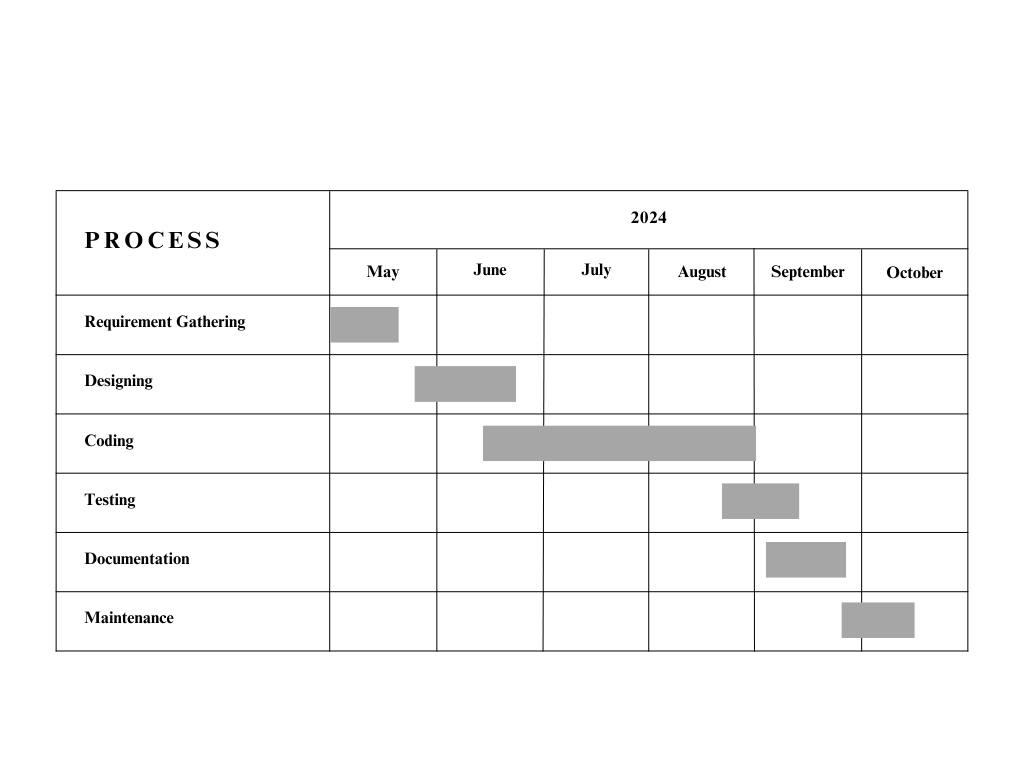
\includegraphics[width=400px]{Diagrams/Gantt_Chart.png}
    \caption{Gantt Chart of Schedule}
\end{figure}
\section{Running the Project}

\begin{itemize}
    \item \textbf{Cloning the Repository}
    \begin{enumerate}[label=\textbf{Step \arabic*:}]
        \item \textbf{Open a Terminal or Command Prompt.}
        \item \textbf{Navigate to the Directory Where You Want to Clone the Repository.}
        \begin{verbatim}
        cd path/to/your/directory
        \end{verbatim}
        \item \textbf{Clone the Repository.}
        \begin{verbatim}
        git clone https://github.com/sushantbramhacharya/
        LabXplorer_Proj.git
        \end{verbatim}
        \item \textbf{Navigate into the Cloned Repository.}
        \begin{verbatim}
        cd LabXplorer_Proj
        \end{verbatim}
    \end{enumerate}
    
    \item \textbf{Restoring the SQL File in pgAdmin}
    \begin{enumerate}[label=\textbf{Step \arabic*:}]
        \item \textbf{Open pgAdmin.}
        \item \textbf{Connect to Your PostgreSQL Server.}
        \begin{itemize}
            \item If you haven’t already set up a server connection, add a new connection using your server credentials.
        \end{itemize}
        \item \textbf{Create a New Database (If Needed).}
        \begin{itemize}
            \item Right-click on the “Databases” node and select “Create > Database...”
            \item Enter a name for your database and click “Save.”
        \end{itemize}
        \item \textbf{Restore the Database from the SQL File.}
        \begin{itemize}
            \item Right-click on your database and select “Restore.”
            \item In the “Restore” dialog, select the “File” tab.
            \item Click the “...” button to browse for the SQL file you want to restore.
            \item Select the SQL file and click “Restore.”
        \end{itemize}
        \item \textbf{Verify the Restoration.}
        \begin{itemize}
            \item Expand the “Schemas” and “Tables” nodes to ensure that your database schema and tables have been correctly restored.
        \end{itemize}
    \end{enumerate}
    
    \item \textbf{Running the Project}
    \begin{enumerate}[label=\textbf{Step \arabic*:}]
        \item \textbf{Ensure Node.js and npm Are Installed.}
        \begin{itemize}
            \item Check if Node.js and npm are installed by running:
            \begin{verbatim}
            node -v
            npm -v
            \end{verbatim}
            \item If not installed, download and install Node.js from \texttt{https://nodejs.org}.
        \end{itemize}
        \item \textbf{Install Project Dependencies.}
        \begin{verbatim}
        npm install
        \end{verbatim}
        \item \textbf{Start the Development Server.}
        \begin{verbatim}
        npm run dev
        \end{verbatim}
        \item \textbf{Access the Application.}
        \begin{itemize}
            \item Open your web browser and go to \texttt{http://localhost:5173} (or the port specified in your project configuration).
        \end{itemize}
    \end{enumerate}
\end{itemize}
\section{Basic Scene in Phaser.js}

Below is a simple example of creating a basic scene using Phaser.js. This scene displays a star image and some text, and logs the pointer coordinates when clicked.

\begin{lstlisting}[language=JavaScript,  basicstyle=\ttfamily, keywordstyle=\color{blue}, commentstyle=\color{green}]
const config = {
    type: Phaser.AUTO,
    width: 800,
    height: 600,
    backgroundColor: '#2d2d2d',
    scene: {
        preload: preload,
        create: create,
        update: update
    }
};
const game = new Phaser.Game(config);
function preload() {
    this.load.image('star', 'https://labs.phaser.io
/assets/sprites/star.png');
}
function create() {
    this.add.image(400, 300, 'star');
    this.add.text(10, 10, 'Hello Phaser!', 
    { font: '24px Arial', fill: '#ffffff' });
    this.input.on('pointerdown', function (pointer) {
        console.log('Pointer down at', pointer.x,
        pointer.y);
    });
}
function update() {
    // Game loop logic
}
\end{lstlisting}
\section{Postgres Database Tables}
\begin{figure}[H]
    \centering
        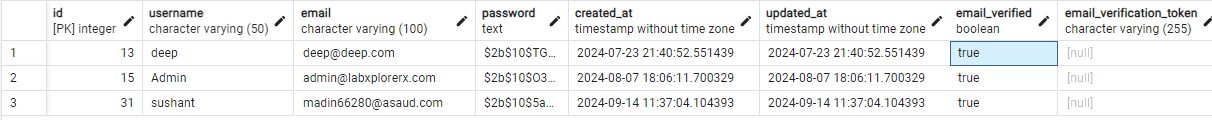
\includegraphics[width=430px]{Diagrams/db/user.png}
    \caption{Table of User}
\end{figure}
\begin{figure}[H]
    \centering
        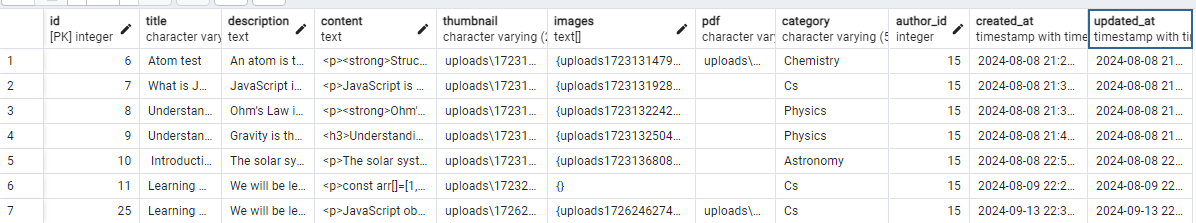
\includegraphics[width=430px]{Diagrams/db/capsules.png}
    \caption{Table of Capsule}
\end{figure}
\begin{figure}[H]
    \centering
        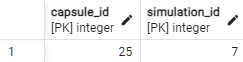
\includegraphics[width=120px]{Diagrams/db/capsule_sim.png}
    \caption{Table of Capsule Simulations}
\end{figure}
\begin{figure}[H]
    \centering
        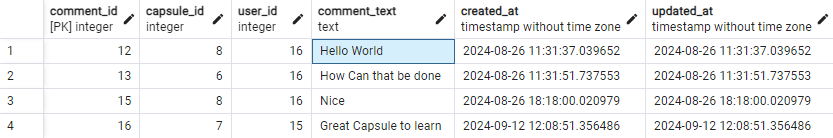
\includegraphics[width=430px]{Diagrams/db/comment.png}
    \caption{Table of Comments}
\end{figure}
\begin{figure}[H]
    \centering
        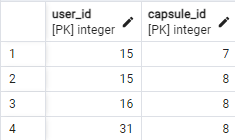
\includegraphics[width=120px]{Diagrams/db/fav.png}
    \caption{Table of Favourites}
\end{figure}
\begin{figure}[H]
    \centering
        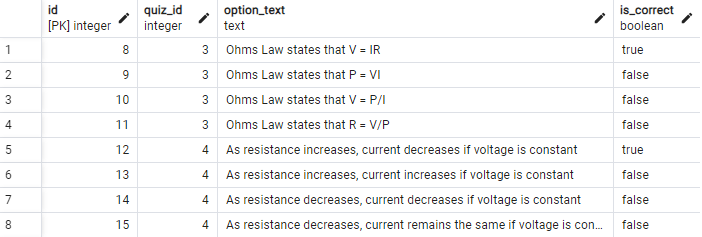
\includegraphics[width=400px]{Diagrams/db/options.png}
    \caption{Table of Quiz Options}
\end{figure}
\begin{figure}[H]
    \centering
        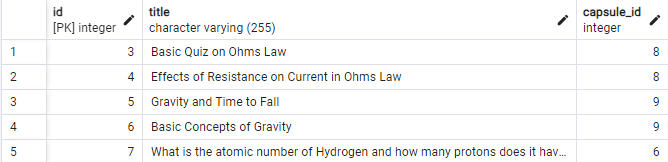
\includegraphics[width=400px]{Diagrams/db/quiz.png}
    \caption{Table of Quizes}
\end{figure}
\begin{figure}[H]
    \centering
        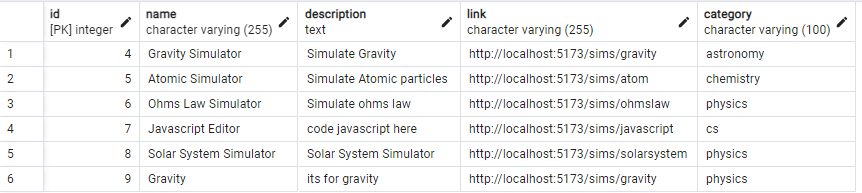
\includegraphics[width=430px]{Diagrams/db/sims.png}
    \caption{Table of Simulations}
\end{figure}
\section{Supervisor Consultation Form}
\begin{figure}[H]
    \centering
        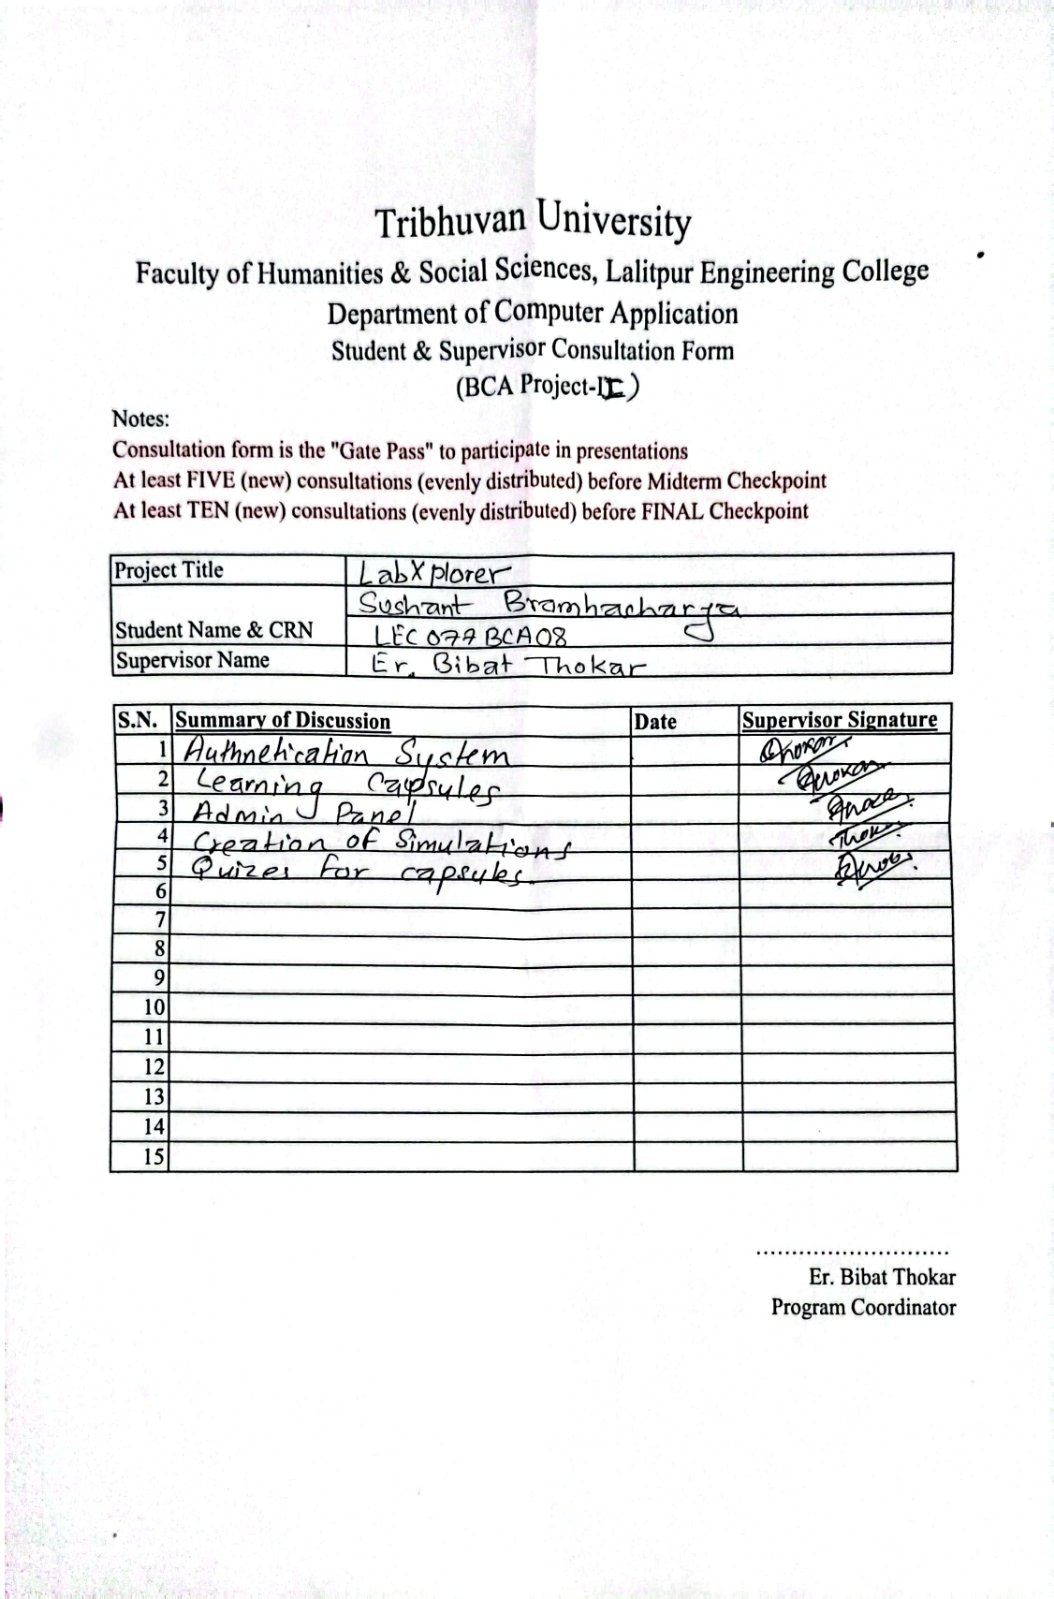
\includegraphics[width=430px]{Diagrams/supervisor.jpg}
    \caption{Supervisor Consultation Form}
\end{figure}